\documentclass{standalone}
\usepackage{tikz}
\usetikzlibrary{patterns, positioning}
\usepackage[sfdefault]{ClearSans} %% option 'sfdefault' activates Clear Sans as the default text font
\usepackage[T1]{fontenc}

\begin{document}
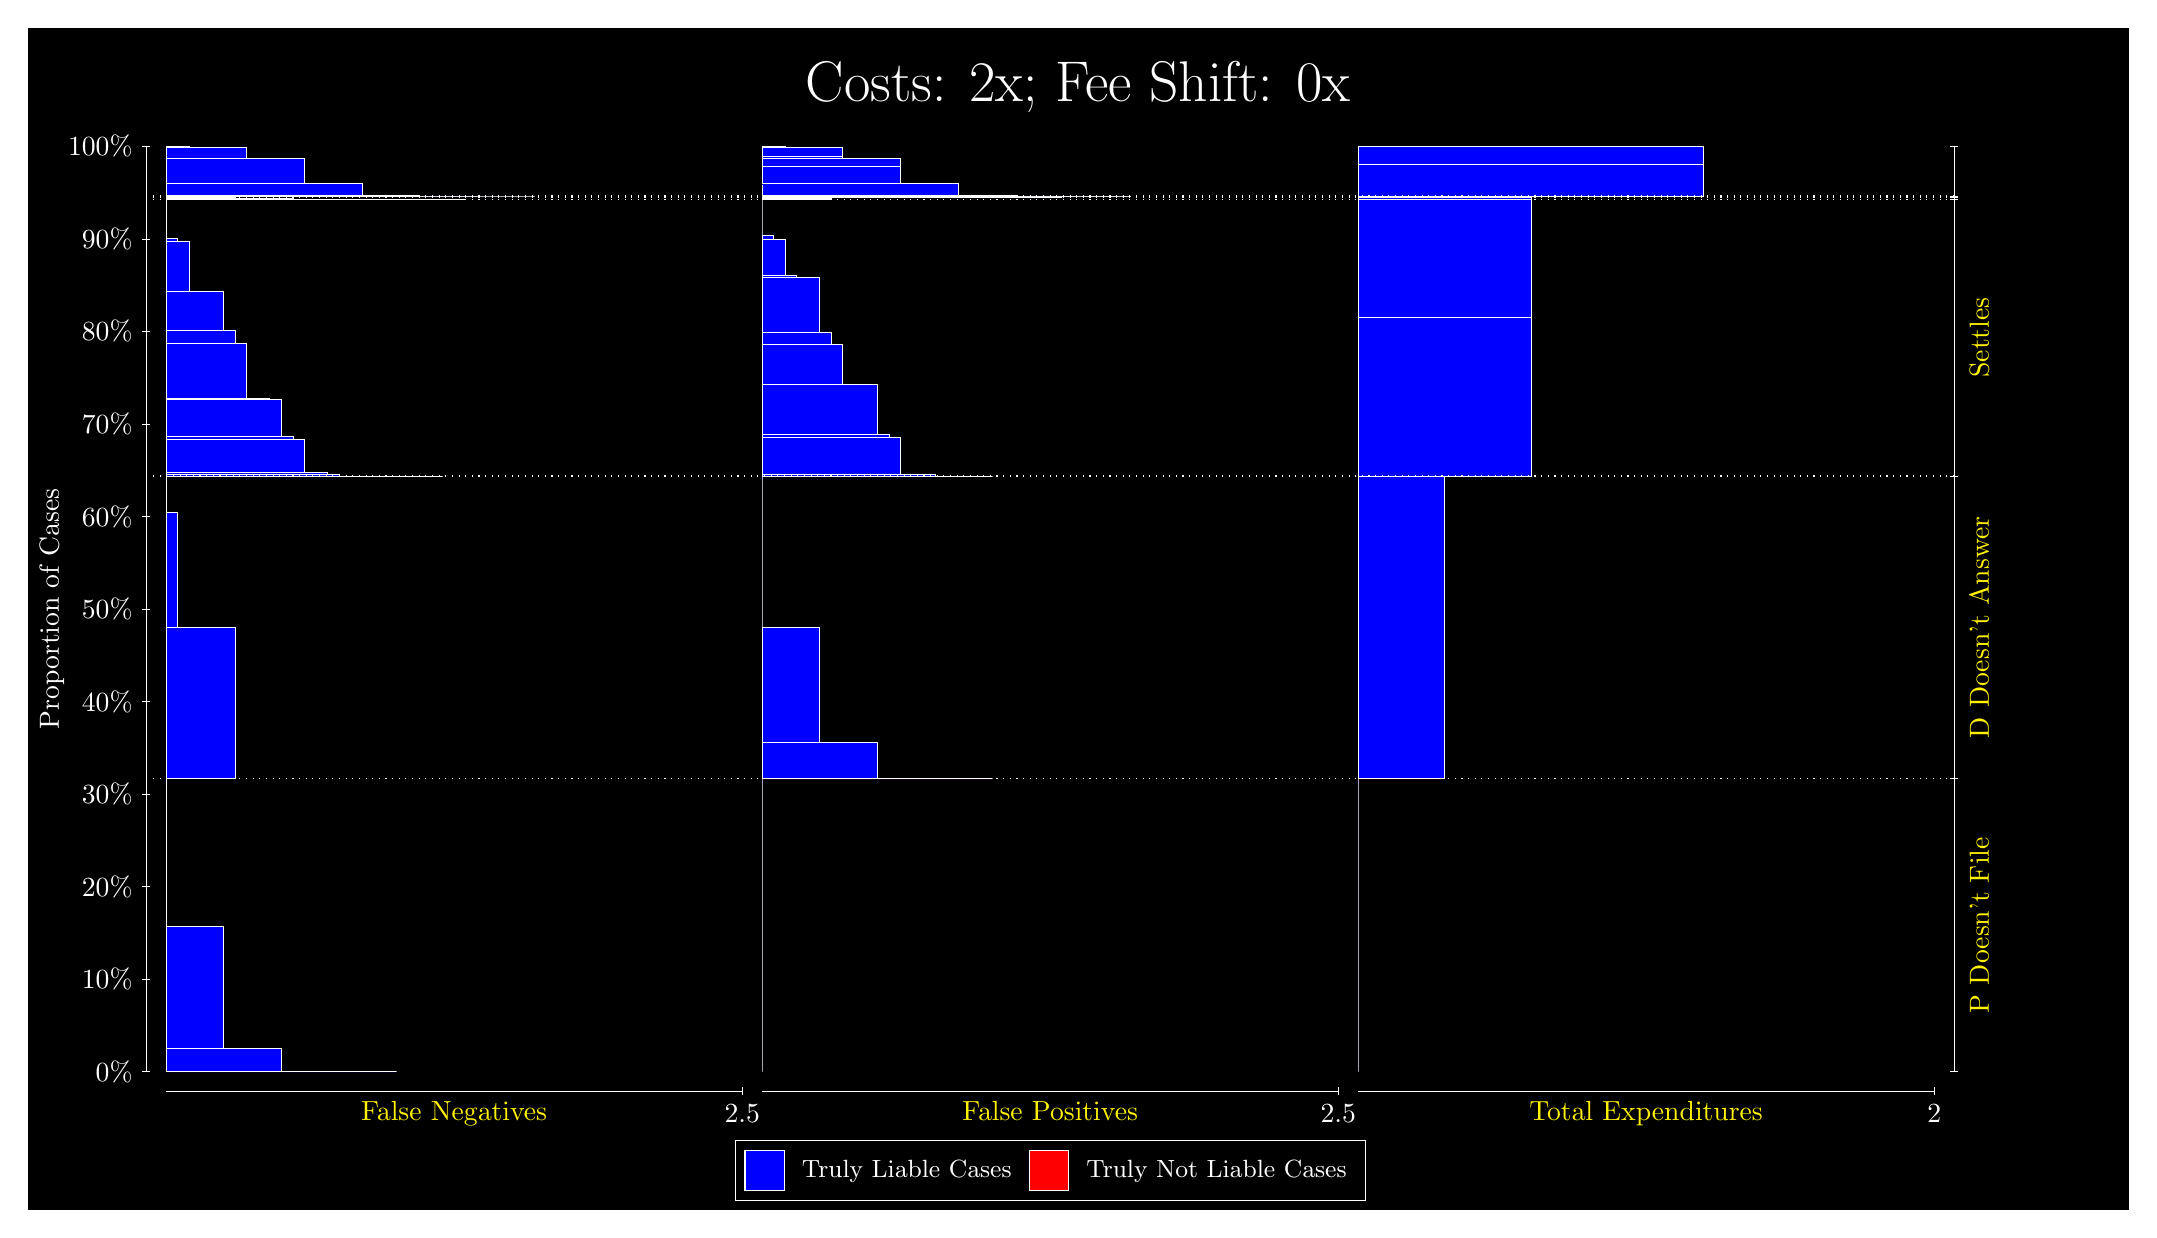
\begin{tikzpicture}
\draw[fill=black] (0,0) rectangle (26.667,15);
\draw[text=white] (0,13.5) rectangle (26.667,15) node[midway] {\huge Costs: 2x; Fee Shift: 0x};
\draw[white, very thin] (1.5,1.75) -- (1.5,13.5);
\node[rotate=90, text=white, anchor=center] at (0.3, 7.625) {Proportion of Cases};
\draw[white, very thin] (1.45,1.75) -- (1.55,1.75);
\node[text=white, anchor=east] at (1.45, 1.75) {0\%};
\draw[white, very thin] (1.45,2.925) -- (1.55,2.925);
\node[text=white, anchor=east] at (1.45, 2.925) {10\%};
\draw[white, very thin] (1.45,4.1) -- (1.55,4.1);
\node[text=white, anchor=east] at (1.45, 4.1) {20\%};
\draw[white, very thin] (1.45,5.275) -- (1.55,5.275);
\node[text=white, anchor=east] at (1.45, 5.275) {30\%};
\draw[white, very thin] (1.45,6.45) -- (1.55,6.45);
\node[text=white, anchor=east] at (1.45, 6.45) {40\%};
\draw[white, very thin] (1.45,7.625) -- (1.55,7.625);
\node[text=white, anchor=east] at (1.45, 7.625) {50\%};
\draw[white, very thin] (1.45,8.8) -- (1.55,8.8);
\node[text=white, anchor=east] at (1.45, 8.8) {60\%};
\draw[white, very thin] (1.45,9.975) -- (1.55,9.975);
\node[text=white, anchor=east] at (1.45, 9.975) {70\%};
\draw[white, very thin] (1.45,11.15) -- (1.55,11.15);
\node[text=white, anchor=east] at (1.45, 11.15) {80\%};
\draw[white, very thin] (1.45,12.325) -- (1.55,12.325);
\node[text=white, anchor=east] at (1.45, 12.325) {90\%};
\draw[white, very thin] (1.45,13.5) -- (1.55,13.5);
\node[text=white, anchor=east] at (1.45, 13.5) {100\%};

\draw[white, very thin] (24.457,1.75) -- (24.457,13.5);
\draw[white, very thin] (24.407,1.75) -- (24.507,1.75);
\node[anchor=west] at (24.407, 1.75) {};
\draw[white, very thin] (24.407,5.4681) -- (24.507,5.4681);
\node[anchor=west] at (24.407, 5.4681) {};
\draw[white, very thin] (24.407,9.3128) -- (24.507,9.3128);
\node[anchor=west] at (24.407, 9.3128) {};
\draw[white, very thin] (24.407,12.83) -- (24.507,12.83);
\node[anchor=west] at (24.407, 12.83) {};
\draw[white, very thin] (24.407,12.853) -- (24.507,12.853);
\node[anchor=west] at (24.407, 12.853) {};
\draw[white, very thin] (24.407,12.869) -- (24.507,12.869);
\node[anchor=west] at (24.407, 12.869) {};
\draw[white, very thin] (24.407,13.5) -- (24.507,13.5);
\node[anchor=west] at (24.407, 13.5) {};

\draw[white, very thin, fill=blue] (1.75,1.75) rectangle (4.6775,1.75);
\draw[white, very thin, fill=blue] (1.75,1.75) rectangle (3.9457,1.7525);
\draw[white, very thin, fill=blue] (1.75,1.7525) rectangle (3.2138,2.0445);
\draw[white, very thin, fill=blue] (1.75,2.0445) rectangle (2.4819,3.5985);
\draw[white, very thin, fill=red] (1.75,3.5985) rectangle (1.75,3.5985);
\draw[white, very thin, fill=blue] (1.75,3.5985) rectangle (1.75,5.4681);
\draw[white, very thin, fill=blue] (1.75,5.4681) rectangle (2.6283,7.3892);
\draw[white, very thin, fill=blue] (1.75,7.3892) rectangle (1.8964,8.8488);
\draw[white, very thin, fill=red] (1.75,8.8488) rectangle (1.75,8.8488);
\draw[white, very thin, fill=blue] (1.75,8.8488) rectangle (1.75,9.3128);
\draw[white, very thin, fill=blue] (1.75,9.3128) rectangle (5.2631,9.3128);
\draw[white, very thin, fill=blue] (1.75,9.3128) rectangle (4.6775,9.3128);
\draw[white, very thin, fill=blue] (1.75,9.3128) rectangle (4.5312,9.3134);
\draw[white, very thin, fill=blue] (1.75,9.3134) rectangle (4.092,9.3144);
\draw[white, very thin, fill=blue] (1.75,9.3144) rectangle (3.9457,9.3322);
\draw[white, very thin, fill=blue] (1.75,9.3322) rectangle (3.7993,9.3574);
\draw[white, very thin, fill=blue] (1.75,9.3574) rectangle (3.5065,9.7773);
\draw[white, very thin, fill=blue] (1.75,9.7773) rectangle (3.3602,9.8194);
\draw[white, very thin, fill=blue] (1.75,9.8194) rectangle (3.2138,10.285);
\draw[white, very thin, fill=blue] (1.75,10.285) rectangle (3.0674,10.304);
\draw[white, very thin, fill=blue] (1.75,10.304) rectangle (2.7746,11.003);
\draw[white, very thin, fill=blue] (1.75,11.003) rectangle (2.6283,11.161);
\draw[white, very thin, fill=blue] (1.75,11.161) rectangle (2.4819,11.659);
\draw[white, very thin, fill=blue] (1.75,11.659) rectangle (2.3355,11.659);
\draw[white, very thin, fill=blue] (1.75,11.659) rectangle (2.0428,12.296);
\draw[white, very thin, fill=blue] (1.75,12.296) rectangle (1.8964,12.335);
\draw[white, very thin, fill=red] (1.75,12.335) rectangle (1.75,12.335);
\draw[white, very thin, fill=blue] (1.75,12.335) rectangle (1.75,12.83);
\draw[white, very thin, fill=blue] (1.75,12.83) rectangle (5.5558,12.83);
\draw[white, very thin, fill=blue] (1.75,12.83) rectangle (4.8239,12.83);
\draw[white, very thin, fill=blue] (1.75,12.83) rectangle (4.092,12.831);
\draw[white, very thin, fill=blue] (1.75,12.831) rectangle (3.3602,12.846);
\draw[white, very thin, fill=blue] (1.75,12.846) rectangle (2.6283,12.853);
\draw[white, very thin, fill=red] (1.75,12.853) rectangle (1.75,12.853);
\draw[white, very thin, fill=blue] (1.75,12.853) rectangle (2.6283,12.859);
\draw[white, very thin, fill=blue] (1.75,12.859) rectangle (1.8964,12.868);
\draw[white, very thin, fill=red] (1.75,12.868) rectangle (1.75,12.868);
\draw[white, very thin, fill=blue] (1.75,12.868) rectangle (1.75,12.869);
\draw[white, very thin, fill=blue] (1.75,12.869) rectangle (6.4341,12.869);
\draw[white, very thin, fill=blue] (1.75,12.869) rectangle (5.7022,12.869);
\draw[white, very thin, fill=blue] (1.75,12.869) rectangle (4.9703,12.879);
\draw[white, very thin, fill=blue] (1.75,12.879) rectangle (4.2384,13.025);
\draw[white, very thin, fill=blue] (1.75,13.025) rectangle (3.5065,13.342);
\draw[white, very thin, fill=blue] (1.75,13.342) rectangle (2.7746,13.488);
\draw[white, very thin, fill=blue] (1.75,13.488) rectangle (2.0428,13.5);
\draw[white, very thin, fill=red] (1.75,13.5) rectangle (1.75,13.5);
\draw[white, very thin, fill=blue] (1.75,13.5) rectangle (1.75,13.5);
\draw[white, very thin, fill=red] (9.3189,1.75) rectangle (9.3189,1.75);
\draw[white, very thin, fill=blue] (9.3189,1.75) rectangle (9.3189,5.4681);
\draw[white, very thin, fill=red] (9.3189,5.4681) rectangle (12.246,5.4681);
\draw[white, very thin, fill=blue] (9.3189,5.4681) rectangle (12.246,5.4681);
\draw[white, very thin, fill=blue] (9.3189,5.4681) rectangle (11.515,5.4789);
\draw[white, very thin, fill=blue] (9.3189,5.4789) rectangle (10.783,5.9321);
\draw[white, very thin, fill=blue] (9.3189,5.9321) rectangle (10.051,7.3917);
\draw[white, very thin, fill=blue] (9.3189,7.3917) rectangle (9.3189,9.3128);
\draw[white, very thin, fill=red] (9.3189,9.3128) rectangle (12.246,9.3128);
\draw[white, very thin, fill=blue] (9.3189,9.3128) rectangle (12.246,9.3128);
\draw[white, very thin, fill=red] (9.3189,9.3128) rectangle (11.661,9.3128);
\draw[white, very thin, fill=blue] (9.3189,9.3128) rectangle (11.661,9.3138);
\draw[white, very thin, fill=blue] (9.3189,9.3138) rectangle (11.515,9.3375);
\draw[white, very thin, fill=red] (9.3189,9.3375) rectangle (11.075,9.3375);
\draw[white, very thin, fill=blue] (9.3189,9.3375) rectangle (11.075,9.8075);
\draw[white, very thin, fill=blue] (9.3189,9.8075) rectangle (10.929,9.8472);
\draw[white, very thin, fill=blue] (9.3189,9.8472) rectangle (10.783,10.484);
\draw[white, very thin, fill=red] (9.3189,10.484) rectangle (10.49,10.484);
\draw[white, very thin, fill=blue] (9.3189,10.484) rectangle (10.49,10.484);
\draw[white, very thin, fill=blue] (9.3189,10.484) rectangle (10.344,10.982);
\draw[white, very thin, fill=blue] (9.3189,10.982) rectangle (10.197,11.14);
\draw[white, very thin, fill=blue] (9.3189,11.14) rectangle (10.051,11.838);
\draw[white, very thin, fill=blue] (9.3189,11.838) rectangle (9.758,11.858);
\draw[white, very thin, fill=blue] (9.3189,11.858) rectangle (9.6116,12.324);
\draw[white, very thin, fill=blue] (9.3189,12.324) rectangle (9.4652,12.366);
\draw[white, very thin, fill=blue] (9.3189,12.366) rectangle (9.3189,12.83);
\draw[white, very thin, fill=red] (9.3189,12.83) rectangle (10.197,12.83);
\draw[white, very thin, fill=blue] (9.3189,12.83) rectangle (10.197,12.837);
\draw[white, very thin, fill=blue] (9.3189,12.837) rectangle (9.4652,12.851);
\draw[white, very thin, fill=blue] (9.3189,12.851) rectangle (9.3189,12.853);
\draw[white, very thin, fill=red] (9.3189,12.853) rectangle (13.125,12.853);
\draw[white, very thin, fill=blue] (9.3189,12.853) rectangle (13.125,12.853);
\draw[white, very thin, fill=blue] (9.3189,12.853) rectangle (12.393,12.853);
\draw[white, very thin, fill=blue] (9.3189,12.853) rectangle (11.661,12.853);
\draw[white, very thin, fill=blue] (9.3189,12.853) rectangle (10.929,12.862);
\draw[white, very thin, fill=blue] (9.3189,12.862) rectangle (10.197,12.869);
\draw[white, very thin, fill=red] (9.3189,12.869) rectangle (14.003,12.869);
\draw[white, very thin, fill=blue] (9.3189,12.869) rectangle (14.003,12.869);
\draw[white, very thin, fill=red] (9.3189,12.869) rectangle (13.271,12.869);
\draw[white, very thin, fill=blue] (9.3189,12.869) rectangle (13.271,12.869);
\draw[white, very thin, fill=red] (9.3189,12.869) rectangle (12.539,12.869);
\draw[white, very thin, fill=blue] (9.3189,12.869) rectangle (12.539,12.88);
\draw[white, very thin, fill=blue] (9.3189,12.88) rectangle (11.807,13.026);
\draw[white, very thin, fill=red] (9.3189,13.026) rectangle (11.807,13.026);
\draw[white, very thin, fill=blue] (9.3189,13.026) rectangle (11.807,13.027);
\draw[white, very thin, fill=blue] (9.3189,13.027) rectangle (11.075,13.246);
\draw[white, very thin, fill=red] (9.3189,13.246) rectangle (11.075,13.246);
\draw[white, very thin, fill=blue] (9.3189,13.246) rectangle (11.075,13.344);
\draw[white, very thin, fill=blue] (9.3189,13.344) rectangle (10.344,13.372);
\draw[white, very thin, fill=blue] (9.3189,13.372) rectangle (10.344,13.49);
\draw[white, very thin, fill=blue] (9.3189,13.49) rectangle (9.6116,13.49);
\draw[white, very thin, fill=blue] (9.3189,13.49) rectangle (9.6116,13.5);
\draw[white, very thin, fill=blue] (9.3189,13.5) rectangle (9.3189,13.5);
\draw[white, very thin, fill=red] (16.888,1.75) rectangle (16.888,1.75);
\draw[white, very thin, fill=blue] (16.888,1.75) rectangle (16.888,5.4681);
\draw[white, very thin, fill=red] (16.888,5.4681) rectangle (17.986,5.4681);
\draw[white, very thin, fill=blue] (16.888,5.4681) rectangle (17.986,9.3128);
\draw[white, very thin, fill=red] (16.888,9.3128) rectangle (19.083,9.3128);
\draw[white, very thin, fill=blue] (16.888,9.3128) rectangle (19.083,11.333);
\draw[white, very thin, fill=red] (16.888,11.333) rectangle (19.083,11.333);
\draw[white, very thin, fill=blue] (16.888,11.333) rectangle (19.083,12.83);
\draw[white, very thin, fill=red] (16.888,12.83) rectangle (19.083,12.83);
\draw[white, very thin, fill=blue] (16.888,12.83) rectangle (19.083,12.853);
\draw[white, very thin, fill=red] (16.888,12.853) rectangle (19.083,12.853);
\draw[white, very thin, fill=blue] (16.888,12.853) rectangle (19.083,12.869);
\draw[white, very thin, fill=red] (16.888,12.869) rectangle (21.279,12.869);
\draw[white, very thin, fill=blue] (16.888,12.869) rectangle (21.279,13.274);
\draw[white, very thin, fill=red] (16.888,13.274) rectangle (21.279,13.274);
\draw[white, very thin, fill=blue] (16.888,13.274) rectangle (21.279,13.5);
\draw[white, dotted] (1.5,5.4681) -- (24.457,5.4681);
\draw[white, dotted] (1.5,9.3128) -- (24.457,9.3128);
\draw[white, dotted] (1.5,12.83) -- (24.457,12.83);
\draw[white, dotted] (1.5,12.853) -- (24.457,12.853);
\draw[white, dotted] (1.5,12.869) -- (24.457,12.869);
\draw[white, very thin] (1.75,1.5) -- (9.0689,1.5);
\node[text=yellow, anchor=north] at (5.4094, 1.5) {False Negatives};
\draw[white, very thin] (9.0689,1.45) -- (9.0689,1.55);
\node[text=white, anchor=north] at (9.0689, 1.45) {2.5};

\draw[white, very thin] (9.3189,1.5) -- (16.638,1.5);
\node[text=yellow, anchor=north] at (12.978, 1.5) {False Positives};
\draw[white, very thin] (16.638,1.45) -- (16.638,1.55);
\node[text=white, anchor=north] at (16.638, 1.45) {2.5};

\draw[white, very thin] (16.888,1.5) -- (24.207,1.5);
\node[text=yellow, anchor=north] at (20.547, 1.5) {Total Expenditures};
\draw[white, very thin] (24.207,1.45) -- (24.207,1.55);
\node[text=white, anchor=north] at (24.207, 1.45) {2};

\node[text=yellow, centered, rotate=90] at (24.777, 3.609) {P Doesn't File};
\node[text=yellow, centered, rotate=90] at (24.777, 7.3904) {D Doesn't Answer};
\node[text=yellow, centered, rotate=90] at (24.777, 11.071) {Settles};




\draw (12.978300999999998,1.5) node[draw=none] (baseCoordinate) {};
\begin{scope}[align=center]
        \matrix[scale=0.5, draw=white, below=0.5cm of baseCoordinate, nodes={draw}, column sep=0.1cm]{
            \node[rectangle, draw, minimum width=0.5cm, minimum height=0.5cm, fill=blue] {}; &
            \node[draw=none, font=\small, text=white] (B) {Truly Liable Cases}; &
            \node[rectangle, draw, minimum width=0.5cm, minimum height=0.5cm, fill=red] {}; &
            \node[draw=none, font=\small, text=white] (B) {Truly Not Liable Cases}; \\
            };
\end{scope}

\end{tikzpicture}
\end{document}